\section{Date: 2026-09-22}
\noindent \textbf{Series ID: ACTLISCOU30029} 

\noindent This series is titled Housing Inventory: Active Listing Count in Flathead County, MT and has a frequency of Monthly. The units are Level and the seasonal adjustment is Not Seasonally Adjusted.The observation start date is 2016-07-01 and the observation end date is 2026-08-01.The popularity of this series is 2. \\ 

\noindent \textbf{Series ID: ITMMARM133S} 

\noindent This series is titled U.S. Imports of Services: Maintenance and Repair Services, not included elsewhere and has a frequency of Monthly. The units are Millions of Dollars and the seasonal adjustment is Seasonally Adjusted.The observation start date is 1999-01-01 and the observation end date is 2026-07-01.The popularity of this series is 1. \\ 

\subsection{Raw Regression}
\noindent Regresses the two series against each other directly. A significant result here can come just as easily from both series sharing a long-run trend as from any real relationship.

\begin{center}
\begin{tabular}{lclc}
\toprule
\textbf{Dep. Variable:}              & value\_fred\_ITMMARM133S & \textbf{  R-squared:         } &     0.123   \\
\textbf{Model:}                      &           OLS            & \textbf{  Adj. R-squared:    } &     0.116   \\
\textbf{Method:}                     &      Least Squares       & \textbf{  F-statistic:       } &     16.76   \\
\textbf{Date:}                       &     Tue, 22 Sep 2026     & \textbf{  Prob (F-statistic):} &  7.76e-05   \\
\textbf{Time:}                       &         15:49:46         & \textbf{  Log-Likelihood:    } &   -747.35   \\
\textbf{No. Observations:}           &             121          & \textbf{  AIC:               } &     1499.   \\
\textbf{Df Residuals:}               &             119          & \textbf{  BIC:               } &     1504.   \\
\textbf{Df Model:}                   &               1          & \textbf{                     } &             \\
\textbf{Covariance Type:}            &        nonrobust         & \textbf{                     } &             \\
\bottomrule
\end{tabular}
\begin{tabular}{lcccccc}
                                     & \textbf{coef} & \textbf{std err} & \textbf{t} & \textbf{P$> |$t$|$} & \textbf{[0.025} & \textbf{0.975]}  \\
\midrule
\textbf{const}                       &     452.9830  &       36.286     &    12.484  &         0.000        &      381.134    &      524.832     \\
\textbf{value\_fred\_ACTLISCOU30029} &       0.1837  &        0.045     &     4.094  &         0.000        &        0.095    &        0.273     \\
\bottomrule
\end{tabular}
\begin{tabular}{lclc}
\textbf{Omnibus:}       & 12.594 & \textbf{  Durbin-Watson:     } &    0.214  \\
\textbf{Prob(Omnibus):} &  0.002 & \textbf{  Jarque-Bera (JB):  } &   14.022  \\
\textbf{Skew:}          &  0.833 & \textbf{  Prob(JB):          } & 0.000902  \\
\textbf{Kurtosis:}      &  3.056 & \textbf{  Cond. No.          } & 2.75e+03  \\
\bottomrule
\end{tabular}
%\caption{OLS Regression Results}
\end{center}

Notes: \newline
 [1] Standard Errors assume that the covariance matrix of the errors is correctly specified. \newline
 [2] The condition number is large, 2.75e+03. This might indicate that there are \newline
 strong multicollinearity or other numerical problems.

\begin{figure}
\centering
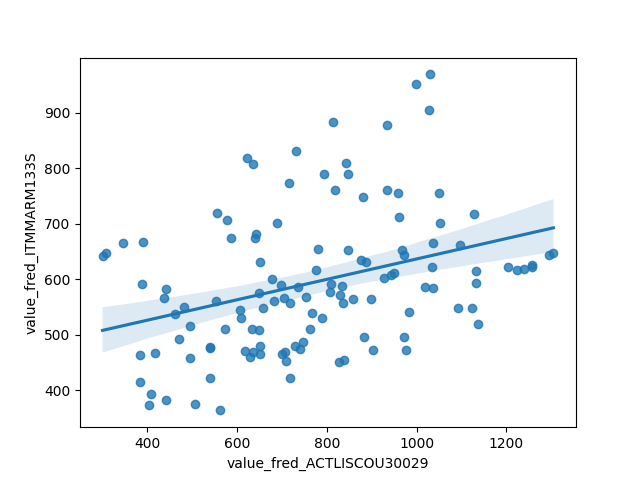
\includegraphics[scale = 0.9]{plots/plot_2026-09-22.png}
\caption{Raw Regression Plot for 2026-09-22}
\end{figure}
\newpage
\subsection{Detrended Regression}
\noindent Regresses the residuals of each series after removing its own linear time trend, so a shared trend can no longer drive the result on its own. A relationship that stays significant here is better evidence of a genuine link between the two series.

\begin{center}
\begin{tabular}{lclc}
\toprule
\textbf{Dep. Variable:}                         & value\_fred\_ITMMARM133S\_detrended & \textbf{  R-squared:         } &     0.195   \\
\textbf{Model:}                                 &                 OLS                 & \textbf{  Adj. R-squared:    } &     0.188   \\
\textbf{Method:}                                &            Least Squares            & \textbf{  F-statistic:       } &     28.77   \\
\textbf{Date:}                                  &           Tue, 22 Sep 2026          & \textbf{  Prob (F-statistic):} &  4.07e-07   \\
\textbf{Time:}                                  &               15:49:46              & \textbf{  Log-Likelihood:    } &   -740.70   \\
\textbf{No. Observations:}                      &                   121               & \textbf{  AIC:               } &     1485.   \\
\textbf{Df Residuals:}                          &                   119               & \textbf{  BIC:               } &     1491.   \\
\textbf{Df Model:}                              &                     1               & \textbf{                     } &             \\
\textbf{Covariance Type:}                       &              nonrobust              & \textbf{                     } &             \\
\bottomrule
\end{tabular}
\begin{tabular}{lcccccc}
                                                & \textbf{coef} & \textbf{std err} & \textbf{t} & \textbf{P$> |$t$|$} & \textbf{[0.025} & \textbf{0.975]}  \\
\midrule
\textbf{const}                                  &   -3.037e-11  &       10.104     & -3.01e-12  &         1.000        &      -20.008    &       20.008     \\
\textbf{value\_fred\_ACTLISCOU30029\_detrended} &       0.2437  &        0.045     &     5.364  &         0.000        &        0.154    &        0.334     \\
\bottomrule
\end{tabular}
\begin{tabular}{lclc}
\textbf{Omnibus:}       &  4.932 & \textbf{  Durbin-Watson:     } &    0.254  \\
\textbf{Prob(Omnibus):} &  0.085 & \textbf{  Jarque-Bera (JB):  } &    5.006  \\
\textbf{Skew:}          &  0.473 & \textbf{  Prob(JB):          } &   0.0819  \\
\textbf{Kurtosis:}      &  2.689 & \textbf{  Cond. No.          } &     222.  \\
\bottomrule
\end{tabular}
%\caption{OLS Regression Results}
\end{center}

Notes: \newline
 [1] Standard Errors assume that the covariance matrix of the errors is correctly specified.

\begin{figure}
\centering
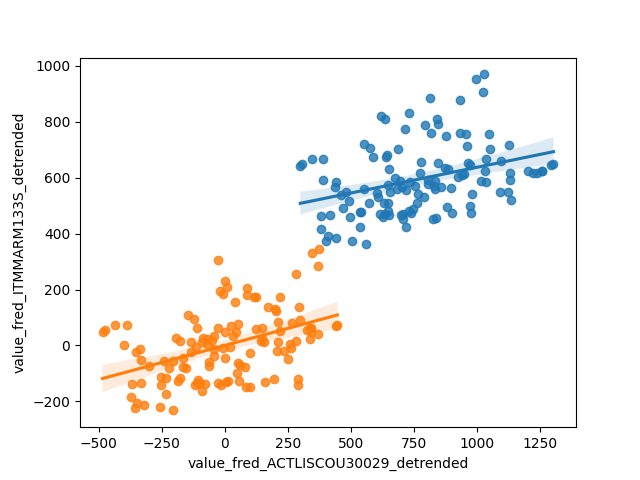
\includegraphics[scale = 0.9]{plots/plot_2026-09-22_detrended.png}
\caption{Detrended Regression Plot for 2026-09-22}
\end{figure}
\newpage
